\chapter{PRBS Modeling and Implementation of Pole Placement Controller}
The aim of this chapter is to do PRBS testing on Single Board Heater System by the application of PRBS signal 
and to design a pole-placement controller. The target group is anyone who has basic knowledge of control engineering. The first half of this chapter is dedicated to do system identification of the SBHS system using the response obtained for a 
PRBS (Pseudo Random Binary Sequence) input. In the second half, a pole-placement controller is designed using this model and 
implemented on SBHS.

\section{PRBS Modelling}

Similar to Chapter \ref{chap1} and \ref{chap2}, we will find the transfer function model of SBHS. 
But there are two major differences. First difference is that we will give a Pseudo Random Binary Sequence to the 
heater input of SBHS and the second difference is that we will find the discrete time transfer function. A Pseudo Random 
Binary Sequence is nothing but a signal whose amplitude varies between two limits randomly at any given time. An 
illustration of the same is given in figure \ref{prbs-fig}. A PRBS signal can be easily generated using the $rand()$ 
function in Scilab. Scilab code to generate the PRBS signal is given at the end of this chapter.

We have used Scilab with Xcos as an interface for sending and receiving data. This interface is shown in figure \ref{prbs-xcos}.
Heater current and fan speed are the two inputs to the system. The heater current is varied with a PRBS signal. A provision
is made to set the parameters like PRBS amplitude and offset value. A provision is also made to time the occurance of the PRBS 
input using a step block. The value of step time in the step block has to be chosen carefully. Sufficient amount of time
should be given to allow the temperature to reach a steady-state before the PRBS signal is applied. In this experiment we are
keeping the fan speed constant at 50\%. The temperature profile thus obtained is the output.


\begin{figure}
\centering
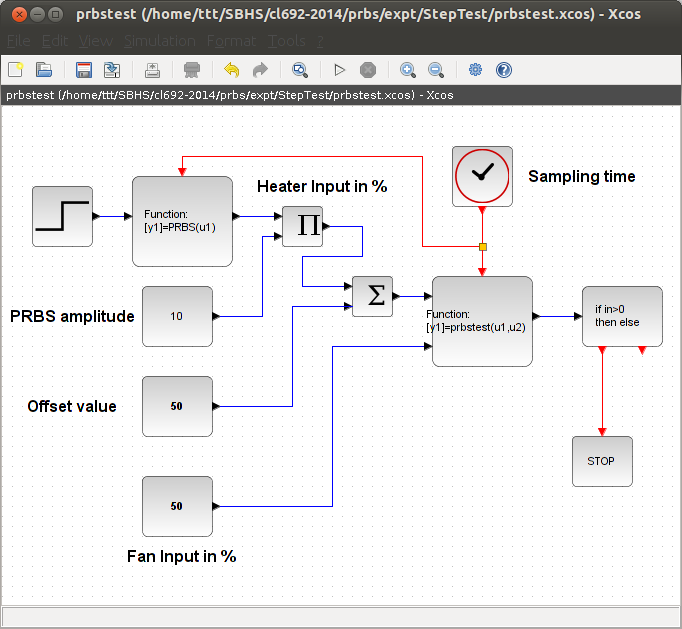
\includegraphics[width=0.7\linewidth]{prbs/prbs-xcos.png}
\caption{Xcos for PRBS testing experiment}
\label{prbs-xcos}
\end{figure}

\subsection{Issues with Step Test and an Alternate Approach}

SBHS is an example of a heater. Suppose you are working in a full scale plant. Current control system designed to control
one of the heaters of the plant is lousy and your supervisor asks you to design a new controller from scratch. The first step
you need to do is identification of the heater transfer function. The catch is, the plant is currently
operational. You can't shut the plant down to identify the heater transfer function. You have to do it while the heater is
operating in the plant. You might think of giving the heater a positive step and measuring the response in the controlled 
temperature. This will increase the temperature of the component being heated for the period of time step is applied. However,
if the process is sensitive to temperature of the component (distillation, for example), it will go off the desired course and
the output of the whole plant will be affected and will be undesirable.\\

There is an alternate approach which is widely used in industry. The input given to the heater for identification is not 
step, but a \textbf{pseudo-random binary sequence (PRBS)}. The concept behind PRBS is that the input is perturbed in such
a way that the time average of the input is the value at which it is being operated currently. Thus, some positive and some
negative steps can be given. This results in some positive and some negative changes in the temperature which leads to the time
average of the performance of the plant remaining the same. Thus, PRBS testing can be done in a working plant without 
affecting the plant performance unlike step testing. A typical PRBS and corresponding plant output is shown in 
figure \ref{sample-prbs}

\begin{figure}[H]
\begin{centering}
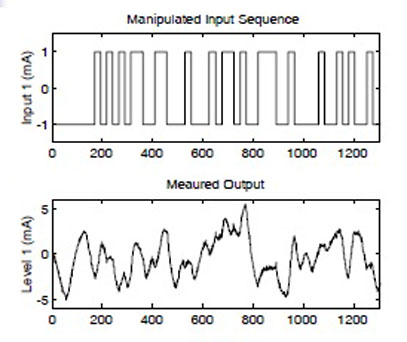
\includegraphics[width=0.6\textwidth]{prbs/PRBS}
\par\end{centering}

\caption{PRBS testing input and output \textit{{[}Image source: CL 686 Advanced
Process Control, Spring 2013-14 lecture slides. Prof. S. C. Patwardhan, IIT Bombay{]}}}
\label{sample-prbs}
\end{figure}

\section{Conducting PRBS Test on SBHS locally}
The detailed procedure to perform a local experiment is explained in Chapter\ref{sercomm}. A summary of the same is provided in section \ref{local-summary} It is same for this section with following changes.

\begin{enumerate}
\item Step1: The working directory is {\tt  prbs/identification}
\item Step2:  Load the functions available in common files directory by executing the command {\tt getd<space>..\textbackslash ..\textbackslash common\_files\ }
\item Step3: Same
\item Step4: Same
\item Step5: Load prbstest function by executing command\\ {\tt exec<space>prbstest.sci}. Load prbs signal generation function by executing command {\tt exec<space>prbs.sci}
\item Step6: Load Xcos code for prbs test using the command\\ {\tt exec<space>prbstest.xcos}
\item Step7: Same
\end{enumerate}

The response is as shown in figure \ref{prbs-test-local}. The data file thus obtained is as shown in the Table \ref{prbs-local-data}. This data file is available for reference in the directory {\tt prbs/identification} with name {\tt prbs-data-local.txt}


\begin{figure}
\centering
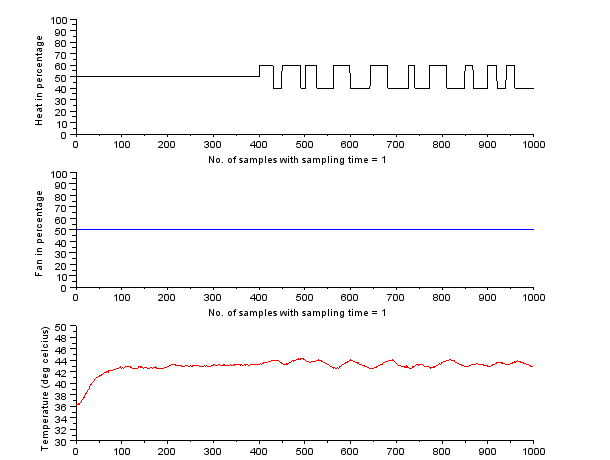
\includegraphics[width=0.7\linewidth]{prbs/prbs-local.png}
\caption{PRBS Local response}
\label{prbs-test-local}
\end{figure}

\begin{table}
\begin{verbatim}
1.0        50.0         50.0       36.4   1417298828422.0
2.0         50.0        50.0      36.2   1417298828525.0
.
 999.0       40.0        50.0        42.9   1417298933585.0
 1000.0     40.0         50.0         42.9   1417298933694.0
\end{verbatim}
\caption{PRBS local experiment data}
\label{prbs-local-data}
\end{table}

\section{Conducting Sine Test on SBHS, virtually}
The detailed procedure to perform a local experiment is explained in Chapter\ref{virtual}. A summary of the same is provided in section \ref{vlabsexpt}. It is same for this section with following changes.

\begin{enumerate}
\item Step1: The working directory is {\tt  prbs/identification}. Open this directory.
\item Step2: Same
\item Step3: Same
\item Step4:  Switch to the working experiment directory and double-click on the file {\tt prbstest.sce}. This will launch scilab and also open the file {\tt prbstest.sce} in the scilab editor. Linux users will have to launch scilab manually. They also have to change the working directory to {\tt  prbs/identification} and then open the {\tt  prbstest.sce} file in the scilab editor.
\item Step5:  Load the functions available in common files directory by executing the command {\tt getd<space>..\textbackslash ..\textbackslash common\_files\ }
\item Step6: Execute the file {\tt prbstest.sce}.  Expect the prbs test xcos diagram to open automatically. If this doesnt happen, check the scilab console for error message.
\item Step7: Execute the prbstest xcos diagram.
\item Step8: Same
\end{enumerate}


 The virtual experiment response is shown in figure \ref{prbs-res}. The corresponding data file is shown in table \ref{prbs-data-virtual}. The time stamps shown are cut short for better viewing. This data file can be found in {\tt prbs/identification} folder for virtual experiments. The name of this file is {\tt prbs-data-virtual.txt}.



\begin{table}
\begin{verbatim}
0 0 100 28.40 14...1731 14...4105 14...4123 14...1763 0.10000E+01
1 50 50 28.30 14...4706 14...7078 14...7096 14...4738 0.10000E+01
.
.
983 40 50 36.70 14...6728 14...9131 14...9148 14...6759 0.98300E+03
984 40 50 36.50 14...7712 14...0115 14...0133 14...7743 0.98400E+03
\end{verbatim}
\caption{Sine data obtained after performing virtual Sine Test}
\label{prbs-data-virtual}
\end{table}


\begin{figure}
\centering
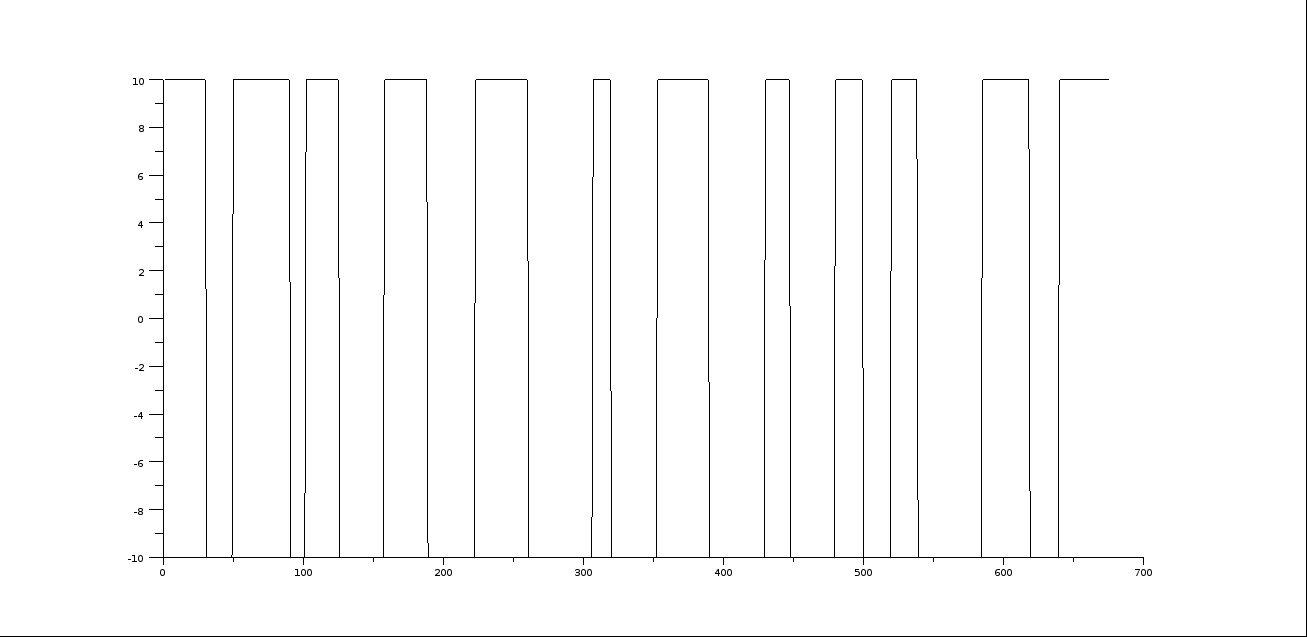
\includegraphics[width=0.7\linewidth]{prbs/prbs-illustration.png}
\caption{A Pseudo Random Binary Sequence}
\label{prbs-fig}
\end{figure}

\begin{figure}
\centering
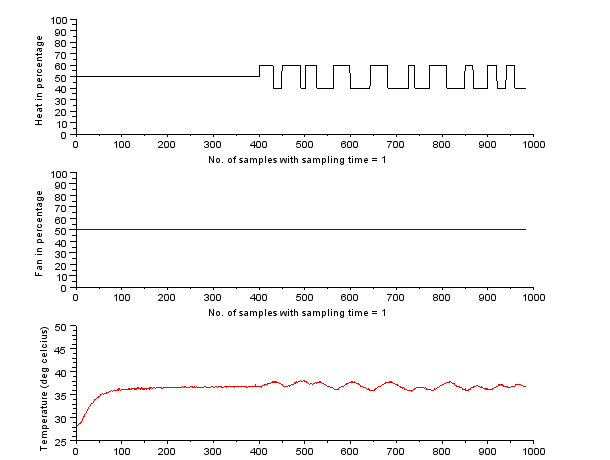
\includegraphics[width=0.7\linewidth]{prbs/prbs-virtual.png}
\caption{PRBS testing response for virtual experiment}
\label{prbs-res}
\end{figure}


\subsection{Determination of Discrete Time Transfer Function models}\label{prbs-model}

System identification is carried out to identify the transfer function between the input signal to the system and output 
from the system. Firstly, a transfer function with unknown parameters is assumed. The system is given a known input and its
response is obtained and then the values of the unknown parameters is chosen such that the sum of squares of the errors is 
minimized. Here, the error is the difference between the actual output and the output predicted by the transfer function model
assumed.
For the given SBHS system, we assume a second order transfer function:

\begin{align}\label{DTF}
G(z)=\frac{b_{1}+b_{2}z^{-1}}{1+a_{1}z^{-1}+a_{2}z^{-2}}z^{-d}
\end{align}


The unknown parameters $a_1, a_2, b_1, b_2$ and $d$ are to be obtained through the response of the system to the known inputs.
$a_1, a_2, b_1, b_2$ are real numbers and $d$ is the plant delay which is an integer.  For these model parameters estimation, we
use a pseudo random binary sequence (PRBS) input. Since the optimization over discrete variables ($d$ in this case) is a very 
difficult routine for computers, we assume a value for $d$ and then optimize over  $a_1, a_2, b_1, b_2$. The optimization 
problem, then, becomes:


\begin{align}
(\hat{b_1}, \hat{b_2}, \hat{a_1}, \hat{a_2})=\underset{b_1, b_2, a_1, a_2}{argmin}\sum_{i=0}^{N}(y(k)-\hat{y}(k))^{2}
\end{align}


Here, $y(k)$ is the output obtained from the system- so it is known. $\hat{y(k)}$ is the estimated output using $y$ the model 
assumed, which can be written as a difference equation:

\begin{align}
\hat{y}(k) = -a_1\hat{y}(k - 1) - a_2\hat{y}(k - 2) + b_1 u(k - d) + b_2 u(k - 1 - d)
\end{align}


\begin{figure}
\centering
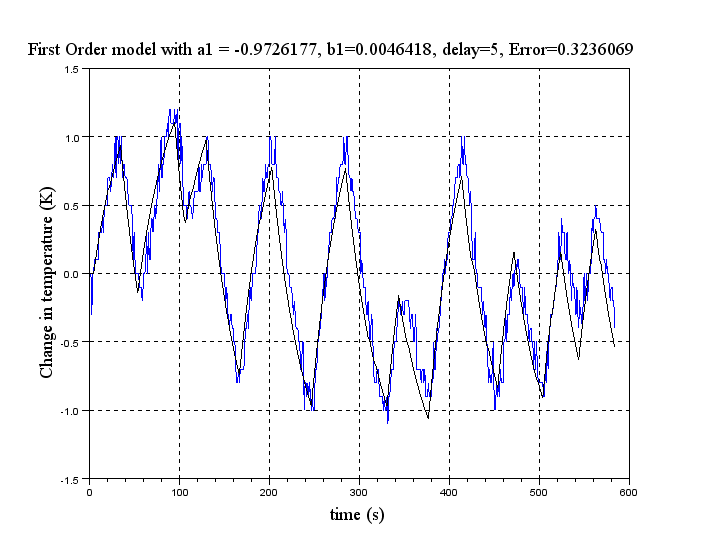
\includegraphics[width=0.7\linewidth]{prbs/prbs-1-fit.png}
\caption{PRBS first order fit}
\label{prbs1-fit}
\end{figure}

\begin{figure}
\centering
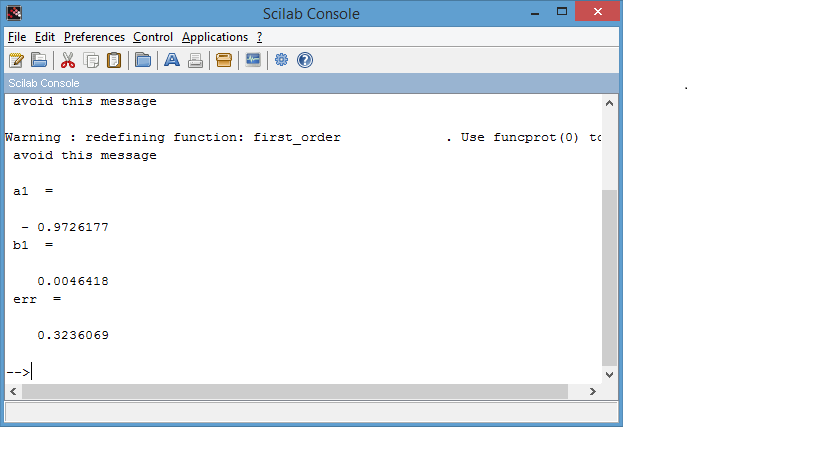
\includegraphics[width=0.7\linewidth]{prbs/prbs-1-model.png}
\caption{PRBS first order model}
\label{prbs-1-model}
\end{figure}

\subsection{Determination of First order Discrete time Transfer Function}
\begin{enumerate}
\item Download the Analysis folder from the sbhs website. It will be available under {\tt downloads} section. The download will be in zip format. Extrat the downloaded zip file. You will get a folder {\tt Analysis}. 
\item Open the {\tt Analysis} folder and then locate and open the folder {\tt Step\_Analysis}.
\item Inside this folder, locate and open the folder {\tt Discrete-order1}
 \item Copy the prbs test data file to this folder.
 \item Start scilab and change the working directory to  {\tt Discrete-order1}
 \item Open the file {\ttfamily optimize.sce} in scilab editor and enter the name of the data file (with extention) in the {\tt filename} field. 
\item Save and run this code and obtain the plot as shown in figure \ref{prbs1-fit}. This plot will also show the first order discrete time transfer function's coefficients a1 and b1.
\item The values are also shown on scilab console as shown in figure \ref{prbs-1-model} 
\end{enumerate}

\begin{align}
\intertext{The results presented are obtained for the data file {\tt prbs-data-virtual.txt}. This data file is present under the {\tt prbs} directory for virtual experiments.The plot thus obtained is reasonably good. See the Scilab plot to get the values of $a1$ and $b1$. 
The figure \ref{prbs1-fit} shows a screen shot of the same. We obtain $a1$ = -0.97, $b1$= 0.004. The transfer function 
obtained here is at the operating point of 50 percentage of heat. If the experiment is repeated at a different operating point, 
the transfer function obtained will be different. The gain will correspondingly be more at a higher operating point. 
This means that the plant is faster at higher temperature. Thus the transfer function of the plant varies with the operating 
point. Let the transfer function we obtain in this experiment be denoted as $G(z)$. We obtain}
G(z)=\frac{0.004}{1-0.97z^{-1}}z^{-5}
\end{align}


\subsection{Determination of Second order Discrete time Transfer Function}
\begin{enumerate}
\item Download the Analysis folder from the sbhs website. It will be available under {\tt downloads} section. The download will be in zip format. Extrat the downloaded zip file. You will get a folder {\tt Analysis}. 
\item Open the {\tt Analysis} folder and then locate and open the folder {\tt Step\_Analysis}.
\item Inside this folder, locate and open the folder {\tt Discrete-order2}
 \item Copy the prbs test data file to this folder.
 \item Start scilab and change the working directory to  {\tt Discrete-order2}
 \item Open the file {\ttfamily optimize.sce} in scilab editor and enter the name of the data file (with extention) in the {\tt filename} field. 
\item Save and run this code and obtain the plot as shown in figure \ref{prbs-2-fit}. This plot will also show the second order discrete time transfer function's coefficients a1, a2, b1 and b2.
\item The values are also shown on scilab console as shown in figure \ref{prbs-2-model} 
\end{enumerate}

\begin{align}
\intertext{The results presented are obtained for the data file {\tt prbs-data-virtual.txt}. This data file is present under the {\tt prbs} directory for virtual experiments.The plot thus obtained is reasonably good. See the Scilab plot to get the values of $a1$, $a2$, $b1$ and $b2$. 
The figure \ref{prbs-2-fit} shows a screen shot of the same. We obtain $a1$ = -1.82, $a2$= 0.833, $b1$ = 0.0017, $b2$= -0.00086, . The transfer function obtained here is at the operating point of 50 percentage of heat. If the experiment is repeated at a different operating point, the transfer function obtained will be different. The gain will correspondingly be more at a higher operating point. 
This means that the plant is faster at higher temperature. Thus the transfer function of the plant varies with the operating 
point. Let the transfer function we obtain in this experiment be denoted as $G(z)$. We obtain}
G(z)=\frac{0.0017 -0.00086z^{-1}}{1-1.826z^{-1}+0.833z^{-2}}z^{-5}
\end{align}


\begin{figure}
\centering
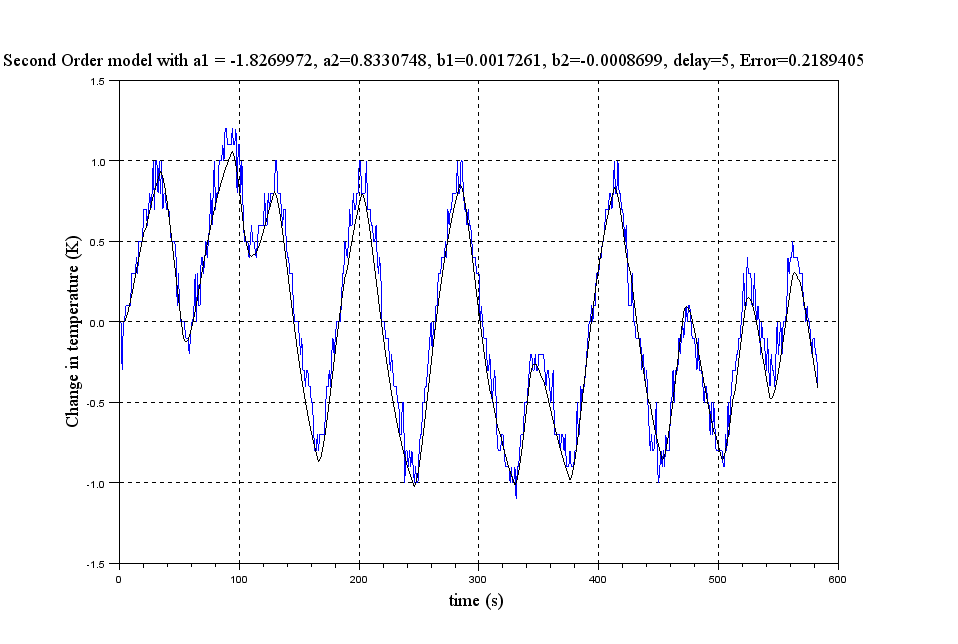
\includegraphics[width=0.7\linewidth]{prbs/prbs-2-fit.png}
\caption{PRBS second order fit}
\label{prbs-2-fit}
\end{figure}

\begin{figure}
\centering
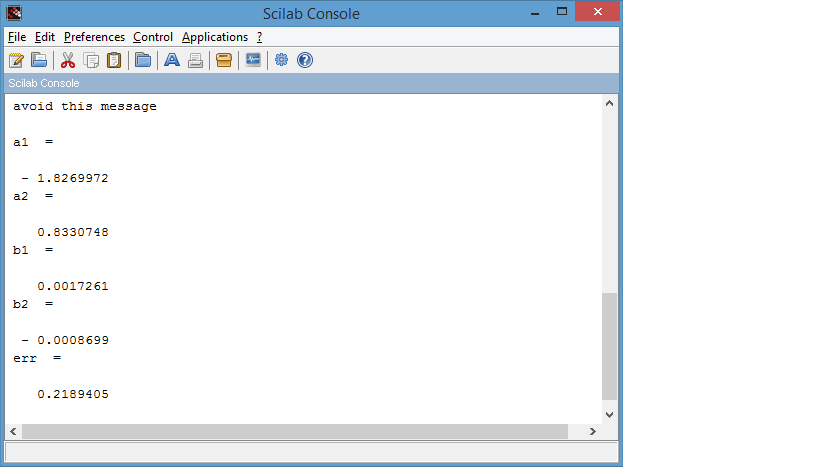
\includegraphics[width=0.7\linewidth]{prbs/prbs-2-model.png}
\caption{PRBS second order model}
\label{prbs-2-model}
\end{figure}


\section{Implementing 2DOF pole-placement controller using PRBS model, virtually}

For deriving the Two degrees of freedom control law, please refer to the chapter \ref{2dof}
The controller was designed for the given transient conditions, rise time = 10 sec, overshoot = 0.1. The experimental result and performance of the controller for setpoint temperature change from 38.00 to 43.00 degree C, i.e. 5 degree C positive step change, has been shown below in Fig \ref{2dof-controller}. The controller designed is not derived for the model explained in earlier sections.

\begin{figure}
\centering
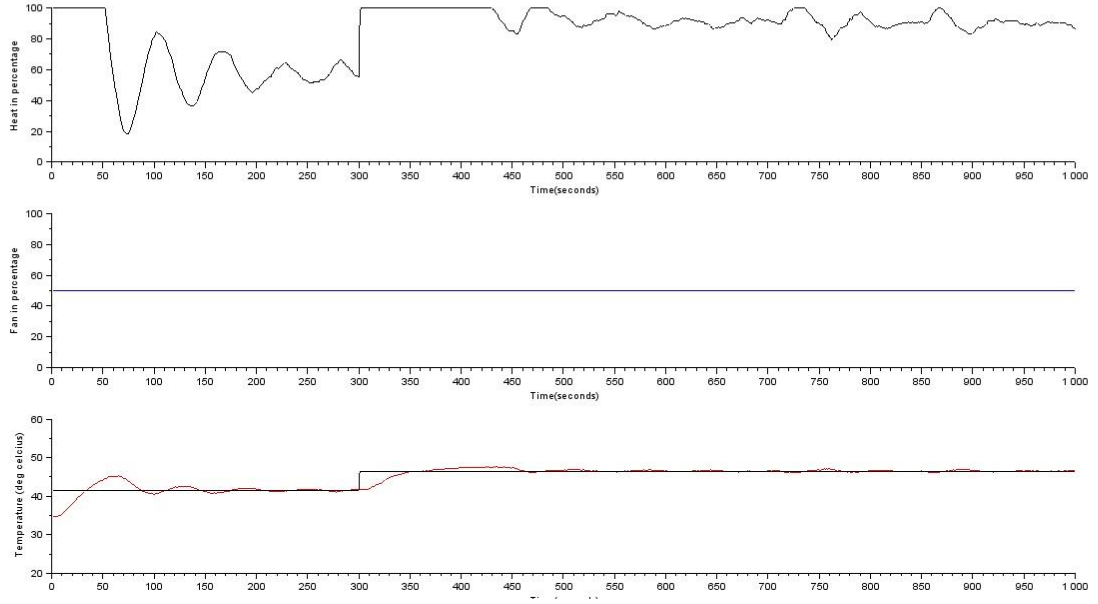
\includegraphics[width=0.9\linewidth]{prbs/prbs-2dof-controller.png}
\caption{2dof controller response}
\label{2dof-controller}
\end{figure}

 The parameters for the 2-DOF pole-placement controller obtained are shown here
\begin{align*}
Tc &= 1 - 1.9444137 z^{ -1} + 0.9447818 z^{ -2}\\
Sc &= 0.0337719 - 0.0656666z^{ -1}+ 0.0319071z^ { -2}\\
Rc &= 10^{-9} (4377900 - 12034140 z^{ -1} + 11094713 z^ {-2} - 3436740.5 z^{-3} + 3.469D^{-09} z ^{-4} \\&- 147850.06 z^ {-5} + 146117.57 z^{ -6} )\\
\gamma &= 0.0337719
\end{align*}

As can be observed from the graph of temperature vs. time (third subplot) in Fig \ref{2dof-controller}, the overshoot criteria was satisfied very easily. The rise time criteria is observed to be more than 30 sec. This can be satisfied with experimentation.
The paramenters are computed by the file {\tt twodof\_para.sce}.  

The steps to be followed to conduct PRBS test experiment virtually remains same as explained in section \ref{vlabsexpt}. only for the following differences
\begin{itemize}
\item Step1: The working directory is {\tt prbs/controller}. Open this directory.
\item Step2: Same
\item Step3: Same
\item Step4:  Switch to the {\tt controller} experiment directory and double-click on the file {\tt prbs.sce}. This will launch scilab and also open the file {\tt prbs.sce} in the scilab editor. Linux users will have to launch scilab manually. They also have to change the working directory to {\tt controller} and then open the {\tt  prbs.sce} file in the scilab editor.
\item Step5:  Load the functions available in common files directory by executing the command {\tt getd<space>..\textbackslash ..\textbackslash common\_files\ }
\item Step6: Execute the file {\tt prbs.sce}.  Expect the prbs test xcos diagram to open automatically. If this doesnt happen, check the scilab console for error message. The values of Rc, Sc, Tc and $\gamma$ are to be entered in the xcos diagram.
\item Step7: Execute the prbstest xcos diagram.
\item Step8: Same
\end{itemize}

\section{Implementing 2DOF pole-placement controller using PRBS model, locally}
The step by step procedure for conducting an experiment locally remains same as explained in section \ref{local-summary} with the following changes
\begin{enumerate}
\item Step1: The working directory is {\tt  prbs/controller}
\item Step2:  Load the functions available in common files directory by executing the command {\tt getd<space>..\textbackslash ..\textbackslash common\_files\ }
\item Step3: Same
\item Step4: Same
\item Step5: Load prbstest function by executing command\\ {\tt exec<space>prbs\_pp.sci}.
\item Step6: Load Xcos code for prbs test using the command\\ {\tt exec<space>prbs\_pp.xcos}.  The values of Rc, Sc, Tc and $\gamma$ are to be entered in the xcos diagram.
\item Step7: Same
\end{enumerate}

\section{Scilab Local codes}\label{prbs-local-codes}
\subsection{Identification codes}
\begin{code}
\ccaption{ser\_init.sce}{\ttfamily ser\_init.sce}
\lstinputlisting{Scilab/local/prbs/identification/ser_init.sce}
\end{code}

\begin{code}
\ccaption{costfunction.sci}{\ttfamily costfunction.sci}
\lstinputlisting{Scilab/local/prbs/identification/costfunction.sci}
\end{code}

\begin{code}
\ccaption{optimize.sce}{\ttfamily optimize.sce}
\lstinputlisting{Scilab/local/prbs/identification/optimize.sce}
\end{code}

\begin{code}
\ccaption{prbs.sci}{\ttfamily prbs.sci}
\lstinputlisting{Scilab/local/prbs/identification/prbs.sci}
\end{code}

\begin{code}
\ccaption{prbstest.sci}{\ttfamily prbstest.sci}
\lstinputlisting{Scilab/local/prbs/identification/prbstest.sci}
\end{code}

\begin{code}
\ccaption{second\_order.sci}{\ttfamily second\_order.sci}
\lstinputlisting{Scilab/local/prbs/identification/second_order.sci}
\end{code}

\begin{code}
\ccaption{start.sce}{\ttfamily start.sce}
\lstinputlisting{Scilab/local/prbs/identification/start.sce}
\end{code}

\subsection{Controller codes}

\begin{code}
\ccaption{prbs.sce}{\ttfamily start.sce}
\lstinputlisting{Scilab/local/prbs/controller/prbs.sce}
\end{code}

\begin{code}
\ccaption{prbs\_pp.sci}{\ttfamily prbs\_pp.sce}
\lstinputlisting{Scilab/local/prbs/controller/prbs_pp.sci}
\end{code}

\begin{code}
\ccaption{ser\_init.sce}{\ttfamily ser\_init.sce}
\lstinputlisting{Scilab/local/prbs/controller/ser_init.sce}
\end{code}

\begin{code}
\ccaption{start.sce}{\ttfamily start.sce}
\lstinputlisting{Scilab/local/prbs/controller/start.sce}
\end{code}

\begin{code}
\ccaption{twodof\_para.sce}{\ttfamily twodof\_para.sce}
\lstinputlisting{Scilab/local/prbs/controller/twodof_para.sce}
\end{code}



\section{Scilab Virtual codes}\label{prbs-virtual-codes}

\subsection{Identification codes}


\begin{code}
\ccaption{costfunction.sci}{\ttfamily costfunction.sci}
\lstinputlisting{Scilab/virtual/prbs/identification/costfunction.sci}
\end{code}


\begin{code}
\ccaption{optimize.sce}{\ttfamily optimize.sce}
\lstinputlisting{Scilab/virtual/prbs/identification/optimize.sce}
\end{code}

\begin{code}
\ccaption{prbs.sci}{\ttfamily prbs.sci}
\lstinputlisting{Scilab/virtual/prbs/identification/prbs.sci}
\end{code}

\begin{code}
\ccaption{prbstest.sci}{\ttfamily prbstest.sci}
\lstinputlisting{Scilab/virtual/prbs/identification/prbstest.sci}
\end{code}

\begin{code}
\ccaption{prbstest.sce}{\ttfamily prbstest.sce}
\lstinputlisting{Scilab/virtual/prbs/identification/prbstest.sce}
\end{code}

\begin{code}
\ccaption{second\_order.sci}{\ttfamily second\_order.sci}
\lstinputlisting{Scilab/virtual/prbs/identification/second_order.sci}
\end{code}

\subsection{Controller codes}

\begin{code}
\ccaption{prbs.sce}{\ttfamily prbs.sce}
\lstinputlisting{Scilab/virtual/prbs/controller/prbs.sce}
\end{code}

\begin{code}
\ccaption{prbscontrol-virtual.sci}{\ttfamily prbscontrol-virtual.sci}
\lstinputlisting{Scilab/virtual/prbs/controller/prbscontrol-virtual.sci}
\end{code}


\begin{code}
\ccaption{twodof\_para.sce}{\ttfamily twodof\_para.sce}
\lstinputlisting{Scilab/virtual/prbs/controller/twodof_para.sce}
\end{code}





%\bibliography{imc} 
